\documentclass[a4paper]{article}

\usepackage{times}
\usepackage{tikz}
\usepackage[margin=0cm]{geometry}
\usepackage{graphicx}
\usepackage{anyfontsize}
\usepackage{fancyhdr}
\usepackage{indentfirst}
\usepackage{amsmath}
\usepackage[spanish]{babel}
\usepackage[utf8]{inputenc}
\usepackage{titlesec}
\usepackage{enumitem}
\usepackage{caption}
\usepackage{booktabs}

\author{}
\date{}
\title{}

\begin{document}
\thispagestyle{empty}

\begin{tikzpicture}[remember picture, overlay]
    \pgftransformshift{\pgfpoint{0cm}{0cm}}
    \draw [line width=2pt](1cm,-1cm) -- (1cm,-27.7cm) -- (14cm, -27.7cm) -- (14cm, -1cm) -- (1cm, -1cm);
    \draw[line width=2pt] (15cm, -27.7cm) -- (19cm,-27.7cm) -- (19cm, -1cm) -- (15cm, -1cm) --  (15cm, -27.7cm);
    \node [line width=2pt] at (17cm, -3.5cm) {
\includegraphics[width=3cm]{../imagenes/utn.png}};
		\node [line width=2pt] at (7.5cm, -7.5cm) {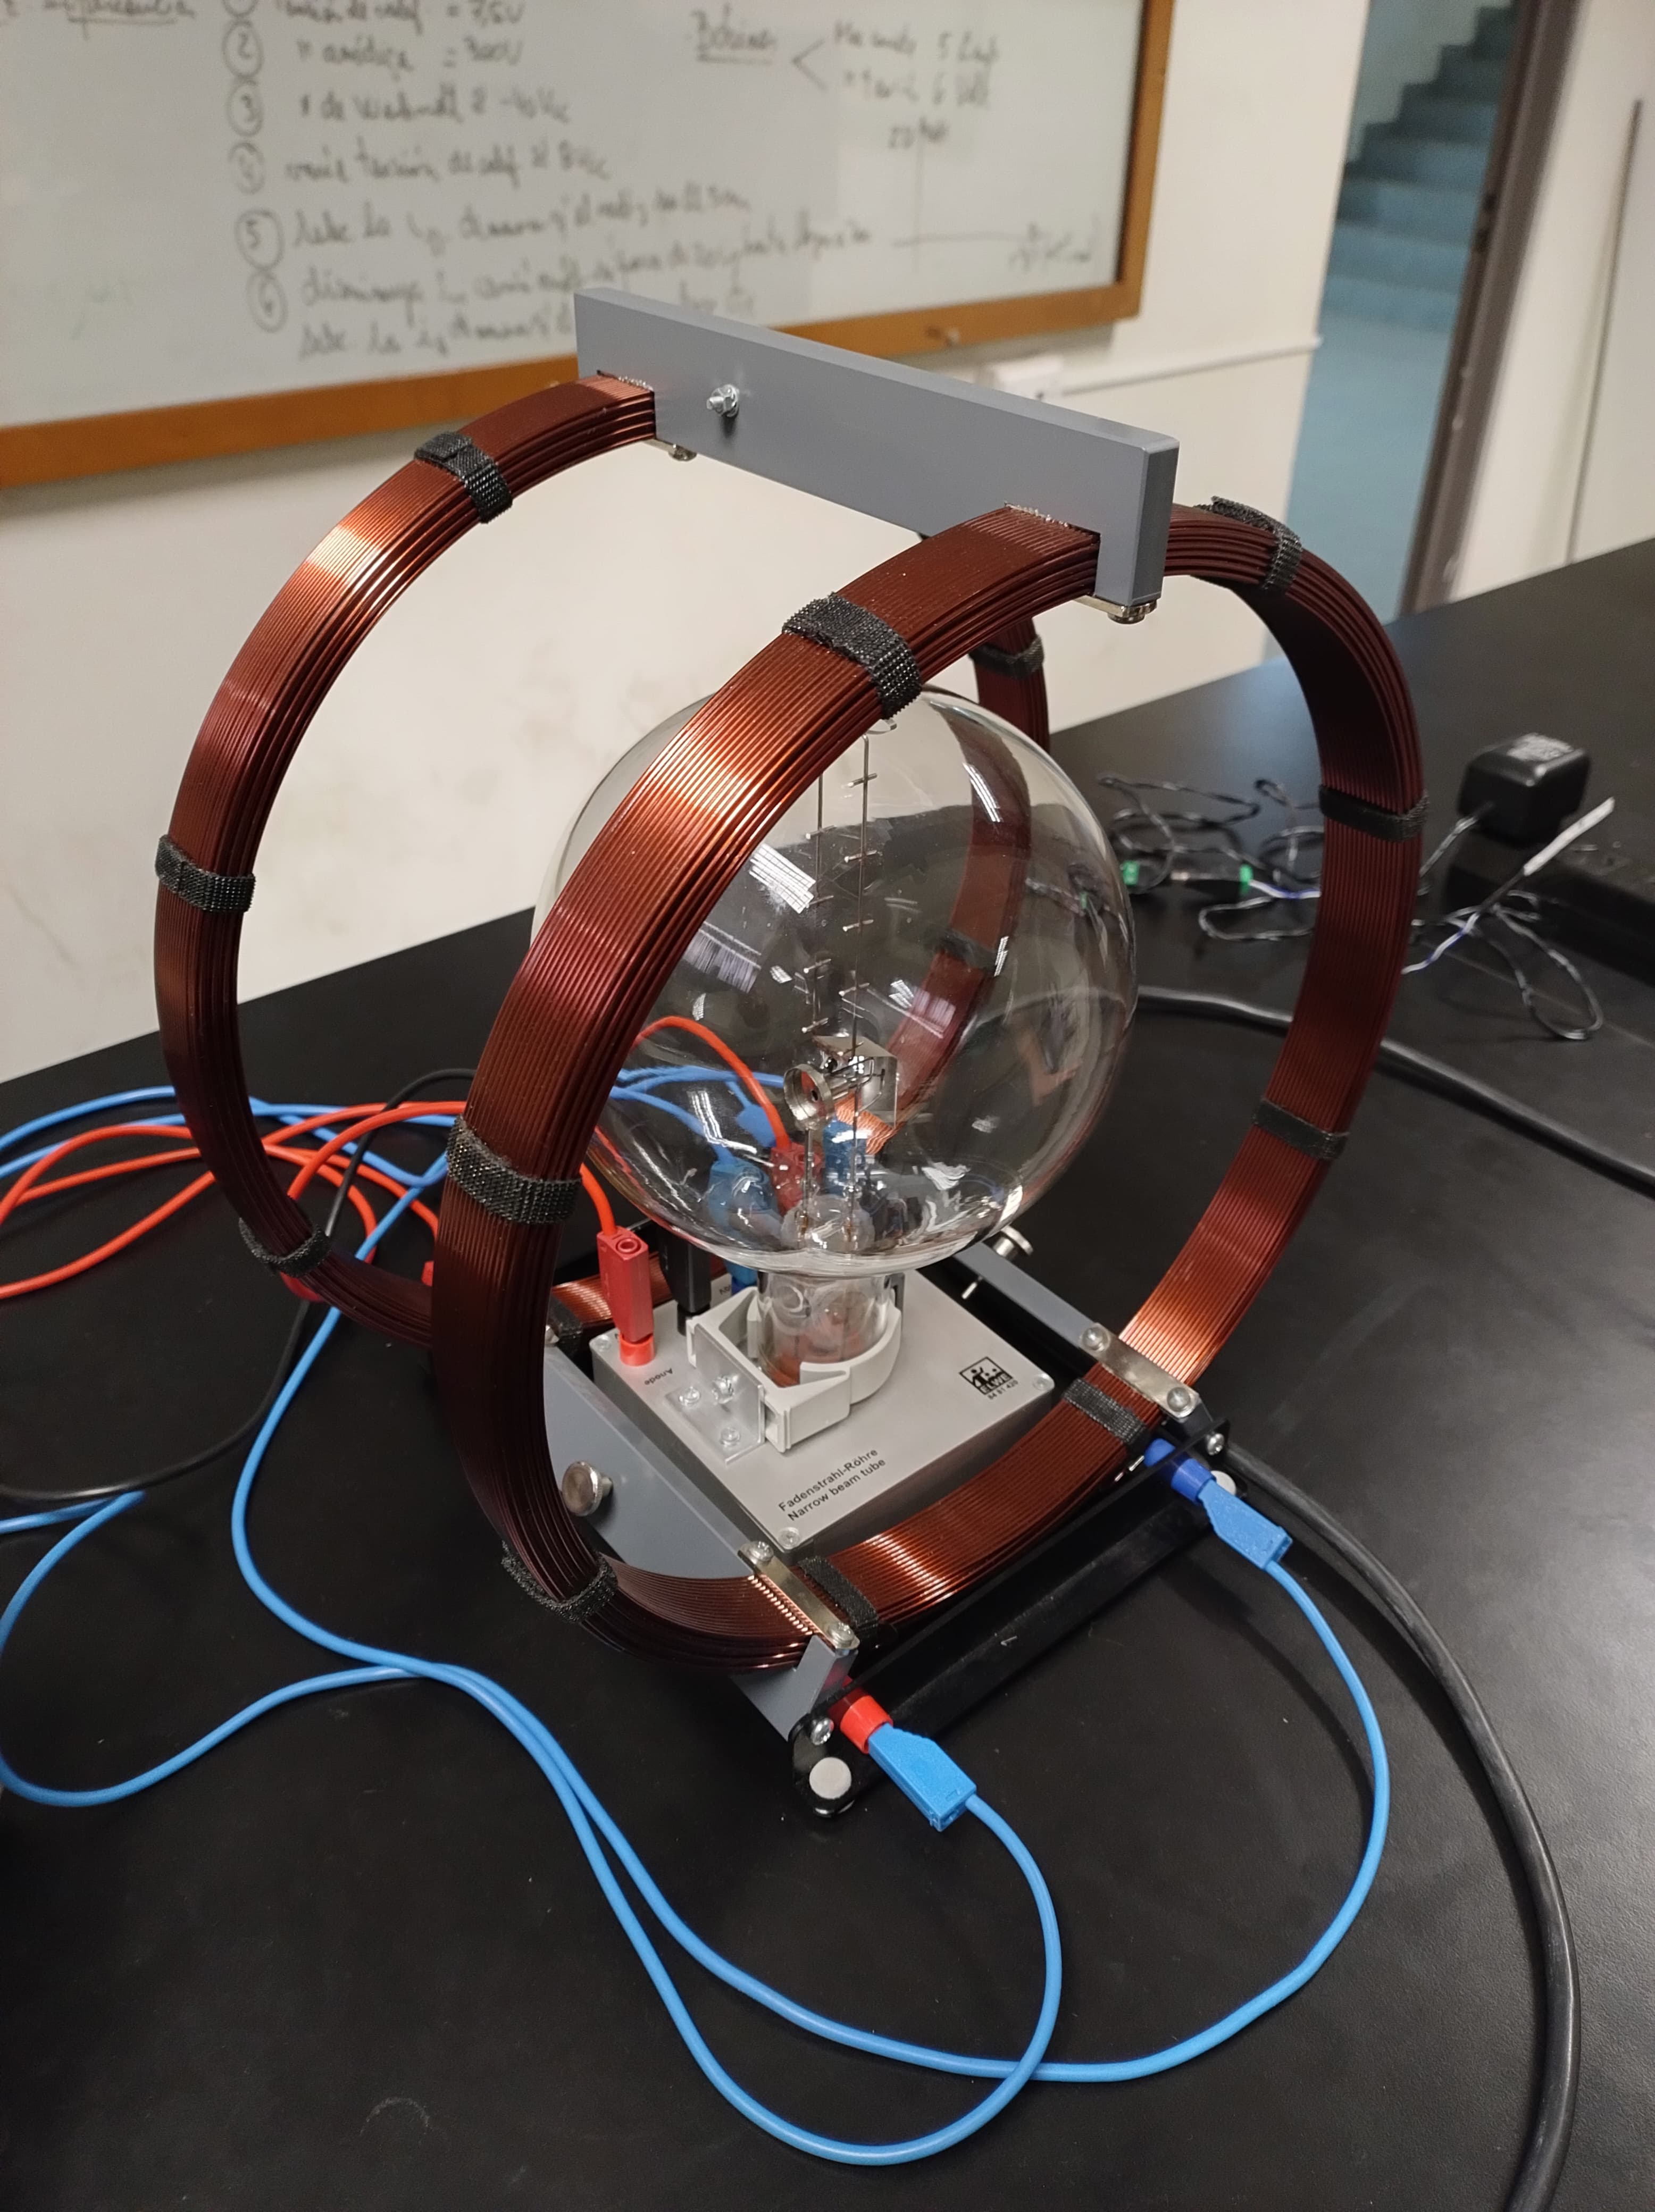
\includegraphics[width=6cm]{../imagenes/ampollaYBobinasHelmholtz.jpeg}};
    \node at (17cm, -7cm) {\scalebox{5}{\textbf{U}}};
    \node at (17cm, -9cm) {\scalebox{5}{\textbf{T}}};
    \node at (17cm, -11cm) {\scalebox{5}{\textbf{N}}};
    \node at (17cm, -14cm) {\scalebox{5}{\textbf{F}}};
    \node at (17cm, -16cm) {\scalebox{5}{\textbf{R}}};
    \node at (17cm, -18cm) {\scalebox{5}{\textbf{C}}};
    \node at (7.5cm, -13cm) {\scalebox{2.5}{\textbf{Carga específica}}};
    \node at (7.5cm, -14cm) {\scalebox{2.5} {\textbf{del electrón}}};

    \node at (7.5cm, -22cm) {
        \begin{minipage}[c]{12cm}
            \begin{itemize}
                \raggedright
                \vspace{1.5cm}
                \item \fontsize{12}{12}\selectfont \textbf{Autores:} \vspace {1mm} \fontsize{11}{12}\selectfont \\
                    \begin{itemize}
                        \item \hspace{2mm} Valentino Rao - Leg. 402308 \\
                        \item \hspace{2mm} Ignacio Ismael Perea - Leg. 406265 \\
                        \item \hspace{2mm} Manuel Leon Parfait - Leg. 406599 \\ 
                        \item \hspace{2mm} Gonzalo Filsinger - Leg. 400460 \\ 
                        \item \hspace{2mm} Agustín Coronel - Leg. 402010 \\
                        \item \hspace{2mm} Marcos Raúl Gatica - Leg. 402006 \\
                    \end{itemize}

                \item \fontsize{12}{12}\selectfont \textbf{Curso:} 2R1. \\
                \item \fontsize{12}{12}\selectfont \textbf{Asignatura:} Física electrónica. \\
                \item \fontsize{12}{12}\selectfont \textbf{Institución:} Universidad Tecnológica Nacional - Facultad Regional de Córdoba \\

            \end{itemize}
        \end{minipage}};

\end{tikzpicture}

\renewcommand{\normalsize}{\fontsize{12}{18}\selectfont}
\newgeometry{margin=1cm}
\fancyhf{}
\renewcommand{\headrulewidth}{0pt}
\renewcommand{\footrulewidth}{0pt}
\fancyfoot[R]{[Rao V. - Parfait M. - Filsinger G. - Perea I. - Coronel A - Gatica M.] [\textbf{pág. \thepage}]}
\setlength{\footskip}{0pt}
\newpage
\thispagestyle{empty}
\text{}

\titleformat{\section} {\fontsize{12}{12}\bfseries}{\thesection.}{0.5em}{\underline}

\newpage
\newpage

\thispagestyle{empty}
\setcounter{page}{0}
\tableofcontents

\newpage
\thispagestyle{fancy}
\twocolumn
\flushbottom
\section{INTRODUCCIÓN}

    \indent El objetivo de este informe es detallar la experiencia de laboratorio llevado a cabo para la medición de la carga específica del electrón.

    \subsection{Fundamentos teóricos}
    \indent La fuerza de Lorentz que afecta al electrón entre cátodo y ánodo, perpendicular al campo $\vec{B}$ generado por las bobinas de Helmholtz y perpendicular a la velocidad, es dada por:

    \begin{center}
        $\vec{F} = e (\vec{v} x \vec{B})$ 
    \end{center}

    \indent Esta fuerza provoca que el electrón adopte una trayectoria orbital, con un cierto radio. \\
    \indent Esto se puede relacionar con la expresión de una fuerza centrípeta que actúa sobre un cuerpo con masa que describe una circunferencia:

    \begin{center}
        $\vec{F} = m {\frac {(\vec{v})^2}{r}}$
    \end{center}

    \indent Ambas expresiones de fuerza son iguales, por lo tanto se puede decir que:

    \begin{center}
        $e \vec{v} \vec{B} = m {\frac {(\vec{v})^2}{r}}$ \\ 
        $e \vec{B} = m \frac {\vec{v}}{r}$
    \end{center}

    \indent Por otro lado, se sabe que la velocidad $\vec{v}$ depende de la tensión de aceleración $U$ del cañón de electrones:

    \begin{align}
        \vec{v} &= [2 (\frac {e}{m}) U]^{\frac{1}{2}} \tag*{} \\[10pt]
        \Rightarrow e \vec{B} &= \frac{m {\vec{v}}}{r} \tag*{} \\[10pt]
        e \vec{B} &= \frac{m[2 (\frac {e}{m}) U]^{\frac{1}{2}}}{r} \tag*{} \\[10pt]
        \frac{e}{m} &= \frac{[2 (\frac {e}{m}) U]^{\frac{1}{2}}}{r \vec{B}} \tag*{} \\[10pt]
        (\frac{e}{m})^{2} &= \frac{[2 (\frac {e}{m}) U]^{\frac{1}{2}}}{r \vec{B}} \tag*{} \\[10pt]
        \frac{e}{m} = \frac{2 U}{(r \vec{B})^2} \tag*{\textit{Carga específica del electrón}}
    \end{align}

    \indent Donde:
    \begin{itemize}
        \item e: carga del electrón.
        \item m: masa del electrón.
        \item U: energía de potencial.
        \item r: radio de la trayectoria circular del electrón.
        \item $\vec{B}$: valor del campo magnético.
    \end{itemize}

\section{ELEMENTOS NECESARIOS}

        \subsection{Tubo de haz finoi - rayos filiformes}

        % PONER UNA FOTO DEL TUBO

       \indent Es una ampolla rellena de neón a cierta presión ajustada precisamente en fábrica, con un cátodo y un ánodo que componen el cañón de electrones junto al cilindro de Wehnelt. Los átomos del gas son ionizados por los choques de los electrones que salen del cañón, el cual origina un rayo luminoso definido. \\
       \indent Se necesita entre 4 a 10 Vcc para calentarse y poder ver el efecto anteriormente mencionado. Además, se puede medir el diámetro de la circunferencia formada por el rayo de electrones usando una escala que trae la ampolla. La distancia entre las marcas de medición es de 20mm, y el diámetro de órbita de haz fino de radiación puede variar de entre 20 a 120mm. \\

    \subsection{Par de bobinas de Helmholtz}

        \begin{figure}[h!]
            \centering
            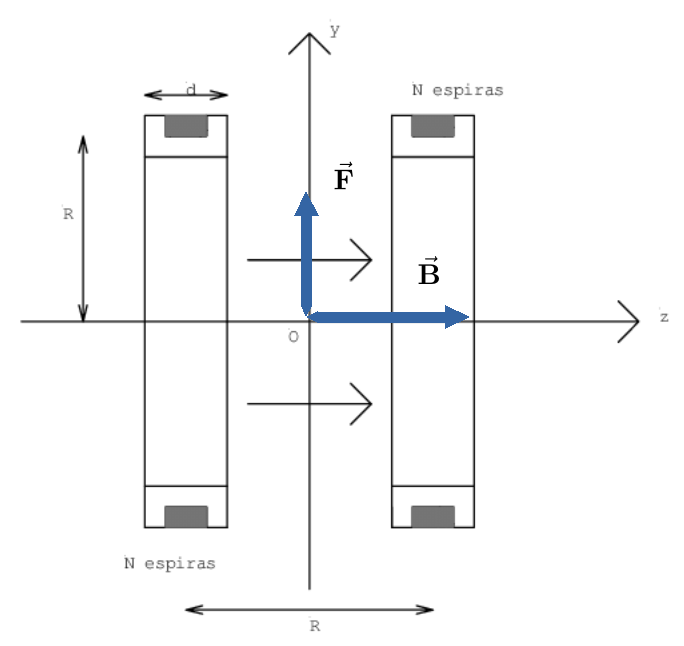
\includegraphics[width = 7.5cm] {../imagenes/dibujoBobinasHelmholtz.png}
        \end{figure}

        \begin{center}
            \textit{Vista lateral izquierda de las bobinas Helmholtz.}
        \end{center}

        \indent Estas bobinas producirán el campo magnético homogéneo entrante. \\

        % PONER UNA FOTO DE LAS BOBINAS

        \indent Lo destacable de este par de bobinas es que el número de espiras es de 124, funciona con una corriente máxima de 5A y una tensión máxima de 6V. \\

    \subsection{Fuente de alimentación para tubos}

    % PONER UNA FOTO DE LA FUENTE

        \indent Lo importante de la fuente usada es que:
        \begin{itemize}
            \item Puede variar la tensión de entre 0 a 300V (para el haz), y otro regulador de 0-50V (calentador).
            \item Permite regular la limitación de corriente entre 0-200mA.
            \item Clavijas de salida 0-300V, y de 0-50V.
            \item Masa común.
        \end{itemize}

    \subsection{Fuente de alimentación (bobinas)} 
    % PONER UNA FOTO DE LA FUENTE

        \indent Lo único importante de esta fuente es poder alimentar de manera estable las bobinas con sus valores de funcionamiento detallados en este índice.
       
\newpage
\noindent
\thispagestyle{fancy}

    \subsection{Multímetro digital}

    %PONER UNA FOTO DEL MULTÍMETRO

        \indent Lo importante de este instrumento es para verificar los voltajes de salida de las fuentes.

\section{MONTAJE}
    \renewcommand{\theenumi}{\roman{enumi}}

    \subsection{Esquema de conexiones}

        \begin{enumerate}
            \item Se colocó el tubo de rayos filiforme entre las bobinas de Helmholtz.

            \textbf{Conexión tubo de haz fino - fuente de alimentación}

            \item Conectar los clavijeros de masa entre sí (negros) de la salida de 50V y de la salida de 12V.
            \item Conectar el polo (+) de la salida de 300V con el ánodo (clavijeros rojos) y el polo negativo con el cátodo (clavijeros negros).
            \item Conectar el voltímetro a la salida de 300V para su medición.
            \item Conectar el polo negativo de la salida de 50V con el cilindro de Wehnelt (clavijeros azules).
            \item Conectar el polo positivo de la salida de 12V con la calefacción de cátodo (clavijeros verdes).
            \item Conectar el clavijero de puesta a tierra de la fuente de alimentación del tubo con el clavijero de tierra del tubo de haz fino de radiación.

            \textbf{Conexión bobinas Helmholtz - fuente de alimentación}

            \item Se conectó las bobinas en serie a la fuente de alimentación con 12 Vcc.
        \end{enumerate}

        \begin{figure}[h!]
            \centering
            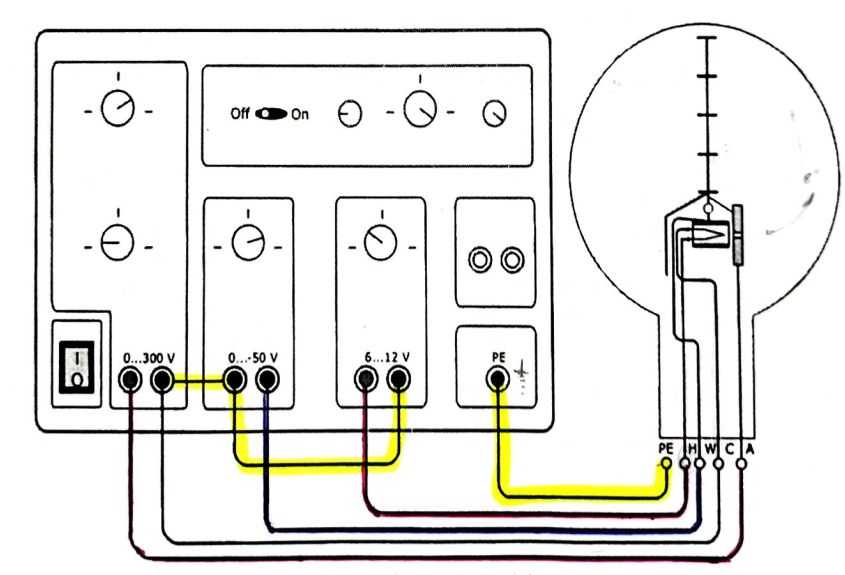
\includegraphics[width = 7cm] {../imagenes/esquemaConexionTuboDeHazFuenteAlim.png}
        \end{figure}

        \begin{center}
            \textit{Conexión Tubo de haz fino - Fuente de alimentación} \\
        \end{center}

        \begin{figure}[h!]
            \centering
            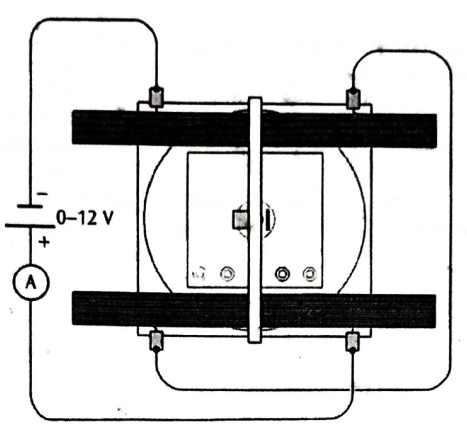
\includegraphics[width = 7cm] {../imagenes/esquemaConexionBobinasHelmholtzFuenteAlim.png}
        \end{figure}

        \begin{center}
            \textit{Conexión Bobinas de Helmholtz - Fuente de alimentación}
        \end{center}

    \subsection{Condiciones en el laboratorio}
        \begin{itemize}
            \item La experiencia se realizó a oscuras.
            \item Se aplicó una tensión de calefacción de: 
            \item Se ajustó la tensión en el ánodo a 300V.
            \item Se reguló la tensión de Wehnelt para que se observe un haz de rayos delgado y definido.
            \item Se hizo variar la corriente de las bobinas ($I_H$) para ver cómo el haz se curva hacia arriba con el fin de medir los radios con la escala en la ampolla.
        \end{itemize}

\section{MEDICIONES}

    \renewcommand{\theenumi}{\roman{enumi}}
    \begin{enumerate}
        \item Se seleccionó la corriente de la bobina de manera que el radio de la órbita circular sea de 5cm y que el haz de electrones quede oculto por la marca de medición.
        \item Se disminuyó la tensión del ánodo de 20 en 20V hasta llegar a $\approx$ 160V. En cada caso, la $I_H$ empleada se ajustó para tener un radio constante.
        \item Se repitió el paso I y II pero con radios que iban disminuyendo cada 0,50cm hasta llegar a un radio de 2cm. \\
    \end{enumerate}

    \begin{center}
        \begin{tabular}{ c  c  c  c }
            \toprule
                 N \textdegree & $I_H$ & Radio & U \\ 
             \midrule
                 1   &   1,4  & 0,064   &   51,7 \\ 
            \bottomrule
        \end{tabular}
    \end{center}

    \indent Con estos datos, fue posible la realización de este gráfico de $2U$ en función de $r^2 (\vec{B})^2$, donde la pendiente de la recta corresponde a la relación $\frac {e}{m}$:

%GRAFICO 2U - r2B2



\end{document}
